\chapter{Descrição do projeto}
\label{c.descricao-do-projeto}

% - Caracterizar claramente o projeto em termos de suas funcionalidades e da forma de sua interação com o usuário e com o ambiente.
% - Apresentar um diagrama em blocos mostrando uma visão geral do sistema a ser desenvolvido.
% - Cada bloco (ou módulo) corresponde a uma representação lógica de uma parte da solução proposta, o qual realiza uma função identificável do sistema completo. Um bloco deve corresponder a uma parte do sistema que pode ser desenvolvida e testada de forma independente das demais.
% - Cada bloco deve será ser descrito individualmente, caracterizar suas entradas e saídas, o processamento que realiza e como se comunica com os demais blocos.
% - Deve ser indicado também, de maneira sucinta, como cada módulo será desenvolvido (se em hardware digital, hardware analógico, software em desktop, firmware embarcado, etc.).

O sistema como um todo segue uma arquitetura cliente-servidor, onde o usuário interage com uma aplicação cliente que, por sua vez, se comunica com um servidor através da internet utilizando algum protocolo de rede. A aplicação cliente, nesse caso, é um aplicativo para dispositivos móveis, enquanto o servidor é uma aplicação monolítica, ou seja, um serviço com \emph{deploy} único que roda em um único processo. Foi considerado o desenvolvimento de vários microserviços, porém a arquiteture monolítica foi escolhida em virtude da simplicidade de desenvolvimento, facilidade de testes e de \emph{deploy}.

\section{Servidor}
\label{s.servidor}

Os princípios do \emph{domain-driven design}, termo cunhado inicialmente por Eric Evans ~\cite{domain-driven-design}, e a ideias propostas por Uncle Bob em \emph{Clean Architecture} ~\cite{clean-architecture} tiveram grande contribuição para o projeto do servidor, tendo em vista que a \emph{separation of concerns} e a divisão da aplicação em camadas bem definidas com um rico modelo de domínio no centro permitem com que a complexidade do projeto cresça de forma manutenível ao longo do tempo.

A partir dos requisitos listados na Seção~\ref{s.requisitos}, se fez necessário identificar os diferentes subdomínios do sistema. Um módulo, também chamado de subdomínio, é um pedaço isolado de código. Como ilustrado pela Figura~\ref{f.system_server}, os seguintes módulos foram identificados:

\begin{itemize}
	\item \texttt{user module}: responsável pelos usuários, gerenciamento de identidade, autenticação e autorização;
	\item \texttt{incident module}: responsável por todas as operações relacionadas aos alertas;
	\item \texttt{notification module}: responsável pelo envio de notificações aos dispositivos dos usuários;
	\item \texttt{shared module}: módulo global para reuso de código entre diferentes módulos.
\end{itemize}

\begin{figure}[h]
	\caption{\small Visão geral do sistema.}
	\centering
	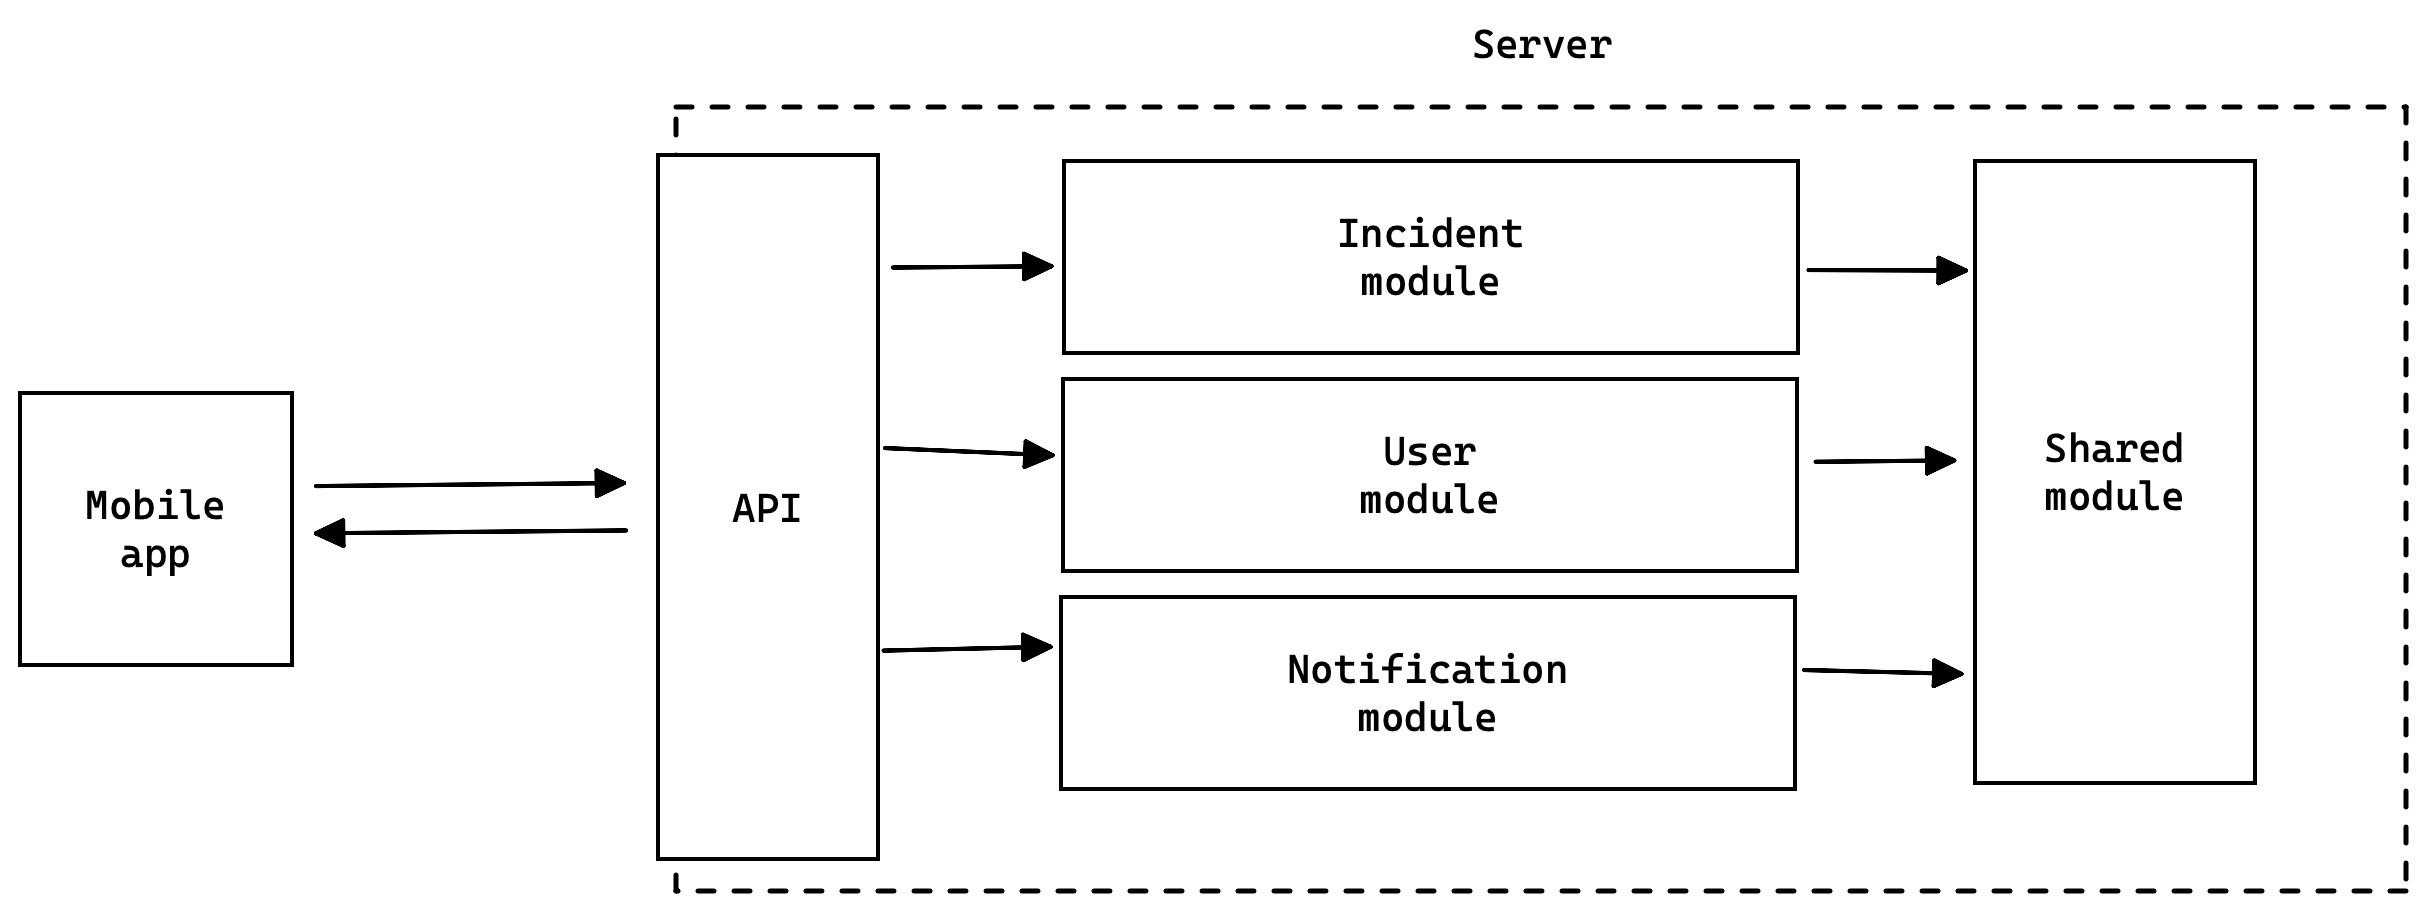
\includegraphics[width=\textwidth]{../diagrams/out/system_server.png}
	\label{f.system_server}
	\legend{\small Fonte: Elaborado pelo autor.}
\end{figure}

\subsection{Camadas dos módulos}

Cada um dos módulos respeita a divisão em camadas descrita pela Figura~\ref{f.system_server_each-module_layers}, onde camadas mais externas dependem das camadas mais internas e, consequentemente, camadas mais internas não conhecem camadas mais externas. 

\begin{figure}[h]
	\caption{\small Camadas de um módulo do servidor.}
	\centering
	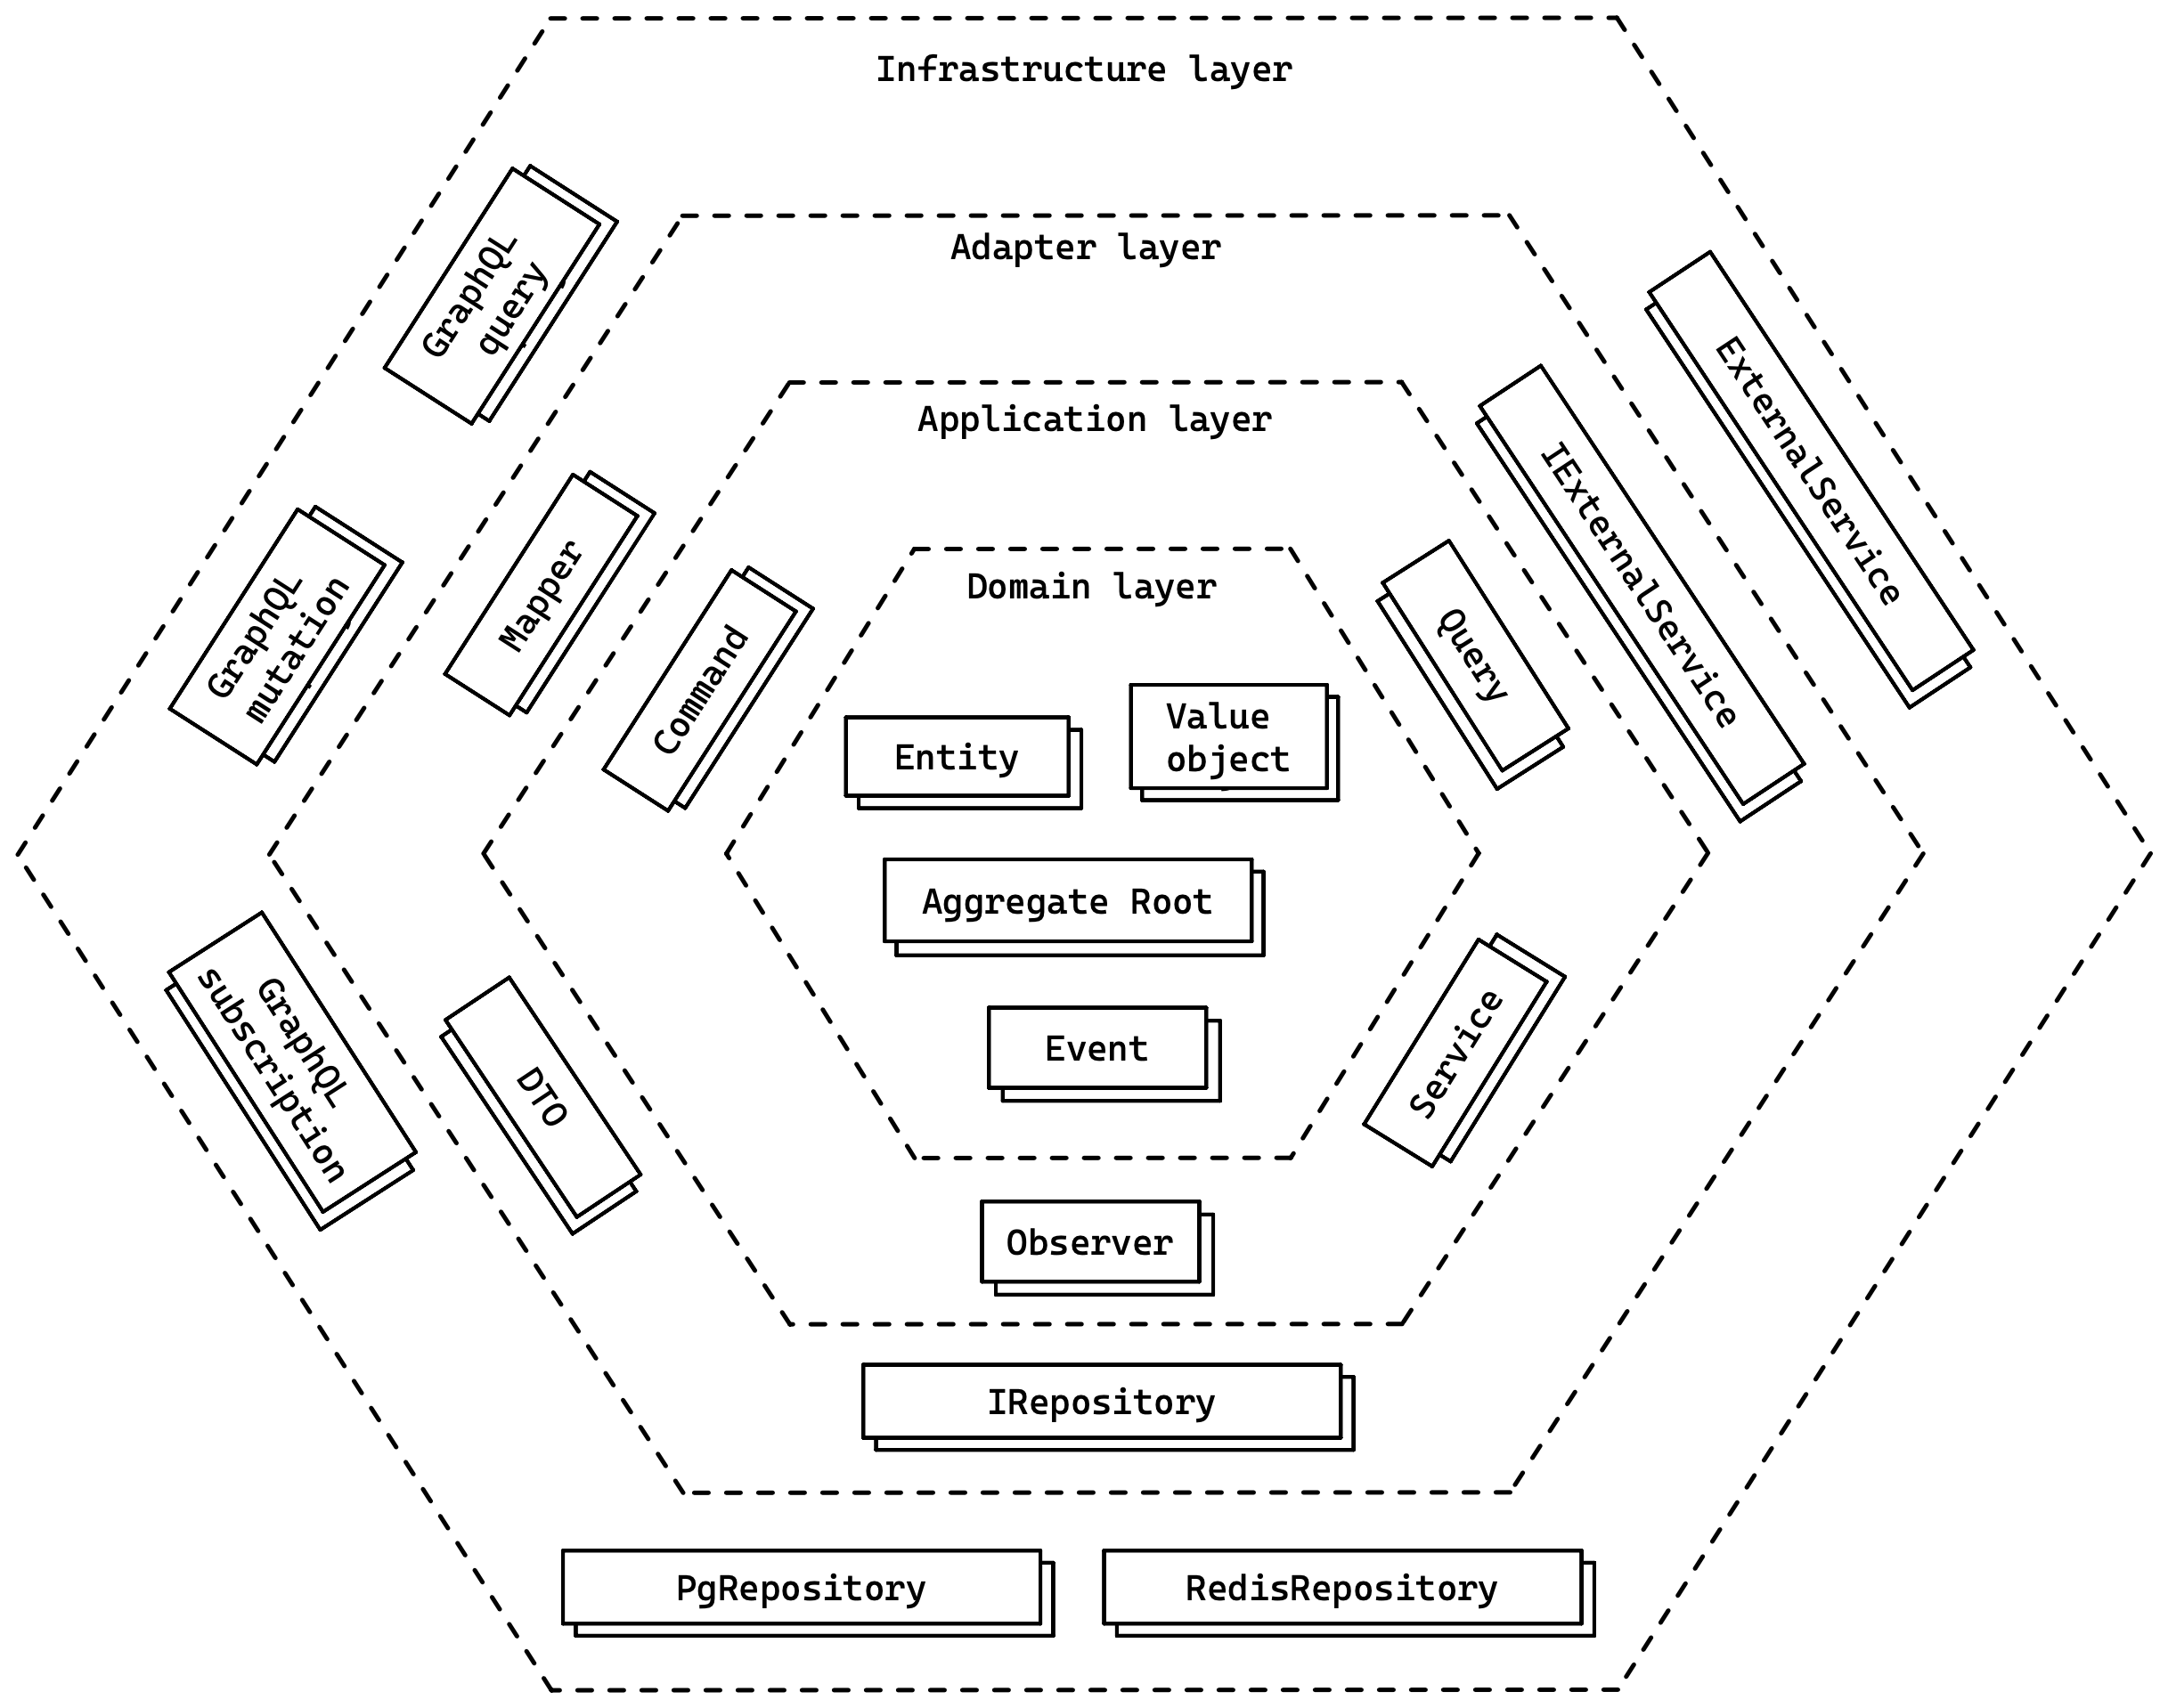
\includegraphics[width=\textwidth]{../diagrams/out/system_server_each-module_layers.png}
	\label{f.system_server_each-module_layers}
	\legend{\small Fonte: Elaborado pelo autor.}
\end{figure}

\subsubsection{A camada de domínio}

A \texttt{domain layer} é a camada mais interna. É a camada que contém tudo aquilo que é importante para o negócio e que está menos propensa a mudar, configurando-se como a camada mais estável dentre todas e a qual todas as outras dependem.

Para encapsular regras de validação, existem os \texttt{value objecs}. Uma \texttt{entity} é um objeto que encorpa um pequeno conjunto de regras de negócio.

Um \texttt{aggregate root} é um tipo específico de \texttt{entity} que pode emitir \texttt{domain events} quando algo relavante para o negócio ocorre, e para isso, ele armazena como estado os eventos que ainda não foram emitidos pela camada de infraestrutura. Ele é implementado pela principal entidade de um \emph{cluster} de \texttt{entities} e \texttt{value objects} relacionados, os quais são tratados como uma única unidade de mudança.

A Figura~\ref{f.system_server_shared-module_domain} demonstra como essas classes abstratas são definidas no módulo \texttt{shared}, além da implementação da classe \texttt{DomainEvents}.

\begin{figure}[h]
	\caption{\small Diagrama de classes da camada de domínio do módulo compartilhado do servidor.}
	\centering
	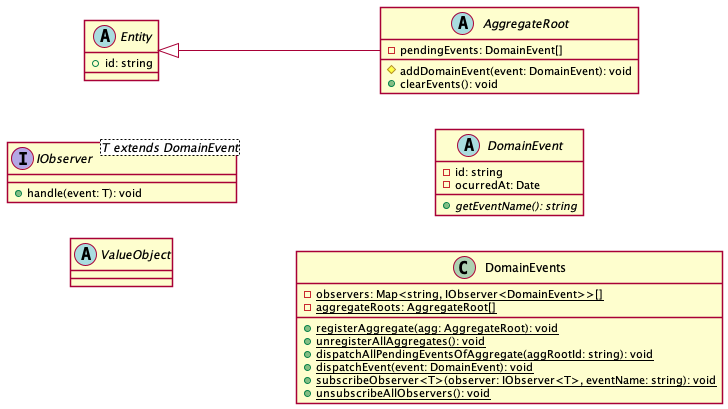
\includegraphics[width=\textwidth]{../diagrams/out/system_server_shared-module_domain.png}
	\label{f.system_server_shared-module_domain}
	\legend{\small Fonte: Elaborado pelo autor.}
\end{figure}

A classe \texttt{DomainEvents} é um \emph{singleton}, ou seja, uma única instância global com tempo de vida vitalício em relação ao tempo de vida da aplicação. Ela é usada para encapsular o estado de quais \texttt{observers} estão interessados em ouvir pelos eventos emitidos por determinados \texttt{aggregate roots}. As instâncias dos \texttt{aggregate roots} inscritos contém \texttt{domain events} que serão dispachados para seus \texttt{observers} quando a camada de infraestrutura persistir as alterações feitas.

\subsubsection{A camada de aplicação}

A \texttt{application layer} contém os casos de uso, ou seja, principais funcionalidades, da aplicação. Em relação ao ambiente externo as entradas são os \texttt{commands} e \texttt{queries}, mas essa camada também implementa \texttt{application services} e \texttt{observers}, que são funções que serão executadas quando um determinado evento de domínio ocorre.

O \emph{Command-Query Separation (CQS)} é um padrão introduzido por Bertrand Meyer ~\cite{object-oriented-software-construction} que afirma que um método é ou um \texttt{command} que executa uma ação ou uma \texttt{query} que retorna dados ao chamador, mas nunca ambos. Dessa forma os fluxos de operações que mudam o sistema (e geram efeitos colaterais) são separados daqueles que apenas requisitam dados ao sistema, tornando o código mais simples de entender e manter.

\subsubsection{A camada de adaptação}

A \texttt{adapter layer} contém abstrações para que a \texttt{application layer} possa interagir com a \texttt{infrastructure layer} sem depender dela. Por exemplo, interfaces de repositórios que acessam bancos de dados, interfaces de classes que chamam APIs externas, mapeadores de objetos entre diferentes camadas (modelo de domínio, DTO, modelo de persistência).

\subsubsection{A camada de infraestrutura}

A \texttt{infrastructure layer} é a camada mais externa. Ela contém os detalhes da aplicação, os quais possuem maior chance de serem trocados por outras bibliotecas ou frameworks específicos ao decorrer do tempo. Isso inclui implementações concretas das abstrações definidas na \texttt{adapter layer} para que elas possam ser executadas em \emph{runtime}, como serviços externos, repositórios para acesso à bancos de dados. Além disso, também contém lógicas de apresentação, como \texttt{HTTP endpoints} e \texttt{GraphQL operations}.

\subsection{Módulos}

Na sequência tem-se uma visão mais ampla de todos os módulos e como eles se inter-relacionam. Um módulo apenas deve se comunicar com outro via eventos de domínio, permitindo o desacoplamento entre eles.

A Figura~\ref{f.system_server_all-modules_domain-entities} ilustra como as entidades de cada módulo estão definidas. 

\begin{figure}[h]
	\caption{\small Entidades de domínio de cada módulo do servidor.}
	\centering
	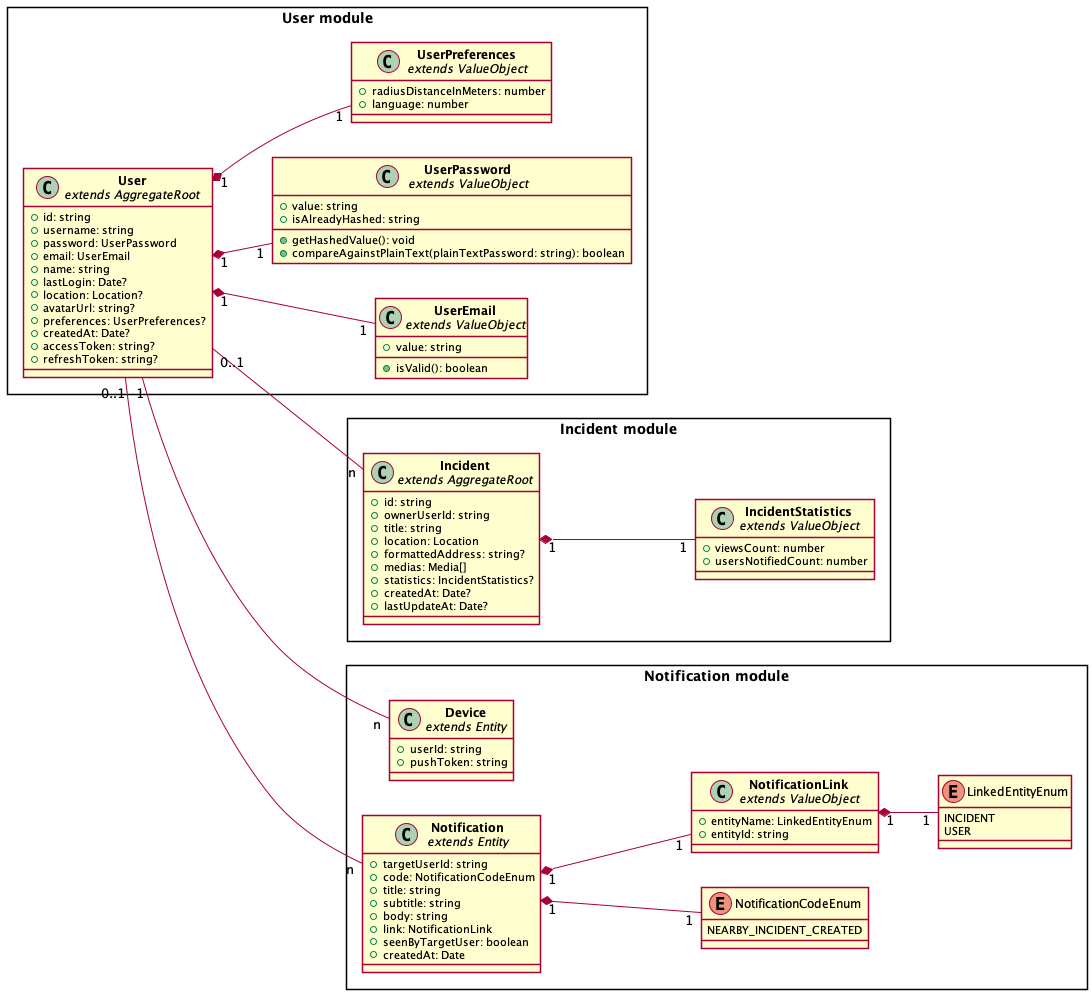
\includegraphics[width=\textwidth]{../diagrams/out/system_server_all-modules_domain-entities.png}
	\label{f.system_server_all-modules_domain-entities}
	\legend{\small Fonte: Elaborado pelo autor.}
\end{figure}

A Figura~\ref{f.system_server_all_modules_commands-observers-events} ilustra as entradas e saídas de cada módulo.

\begin{figure}[h]
	\caption{\small Entradas e saídas de cada módulo do servidor.}
	\centering
	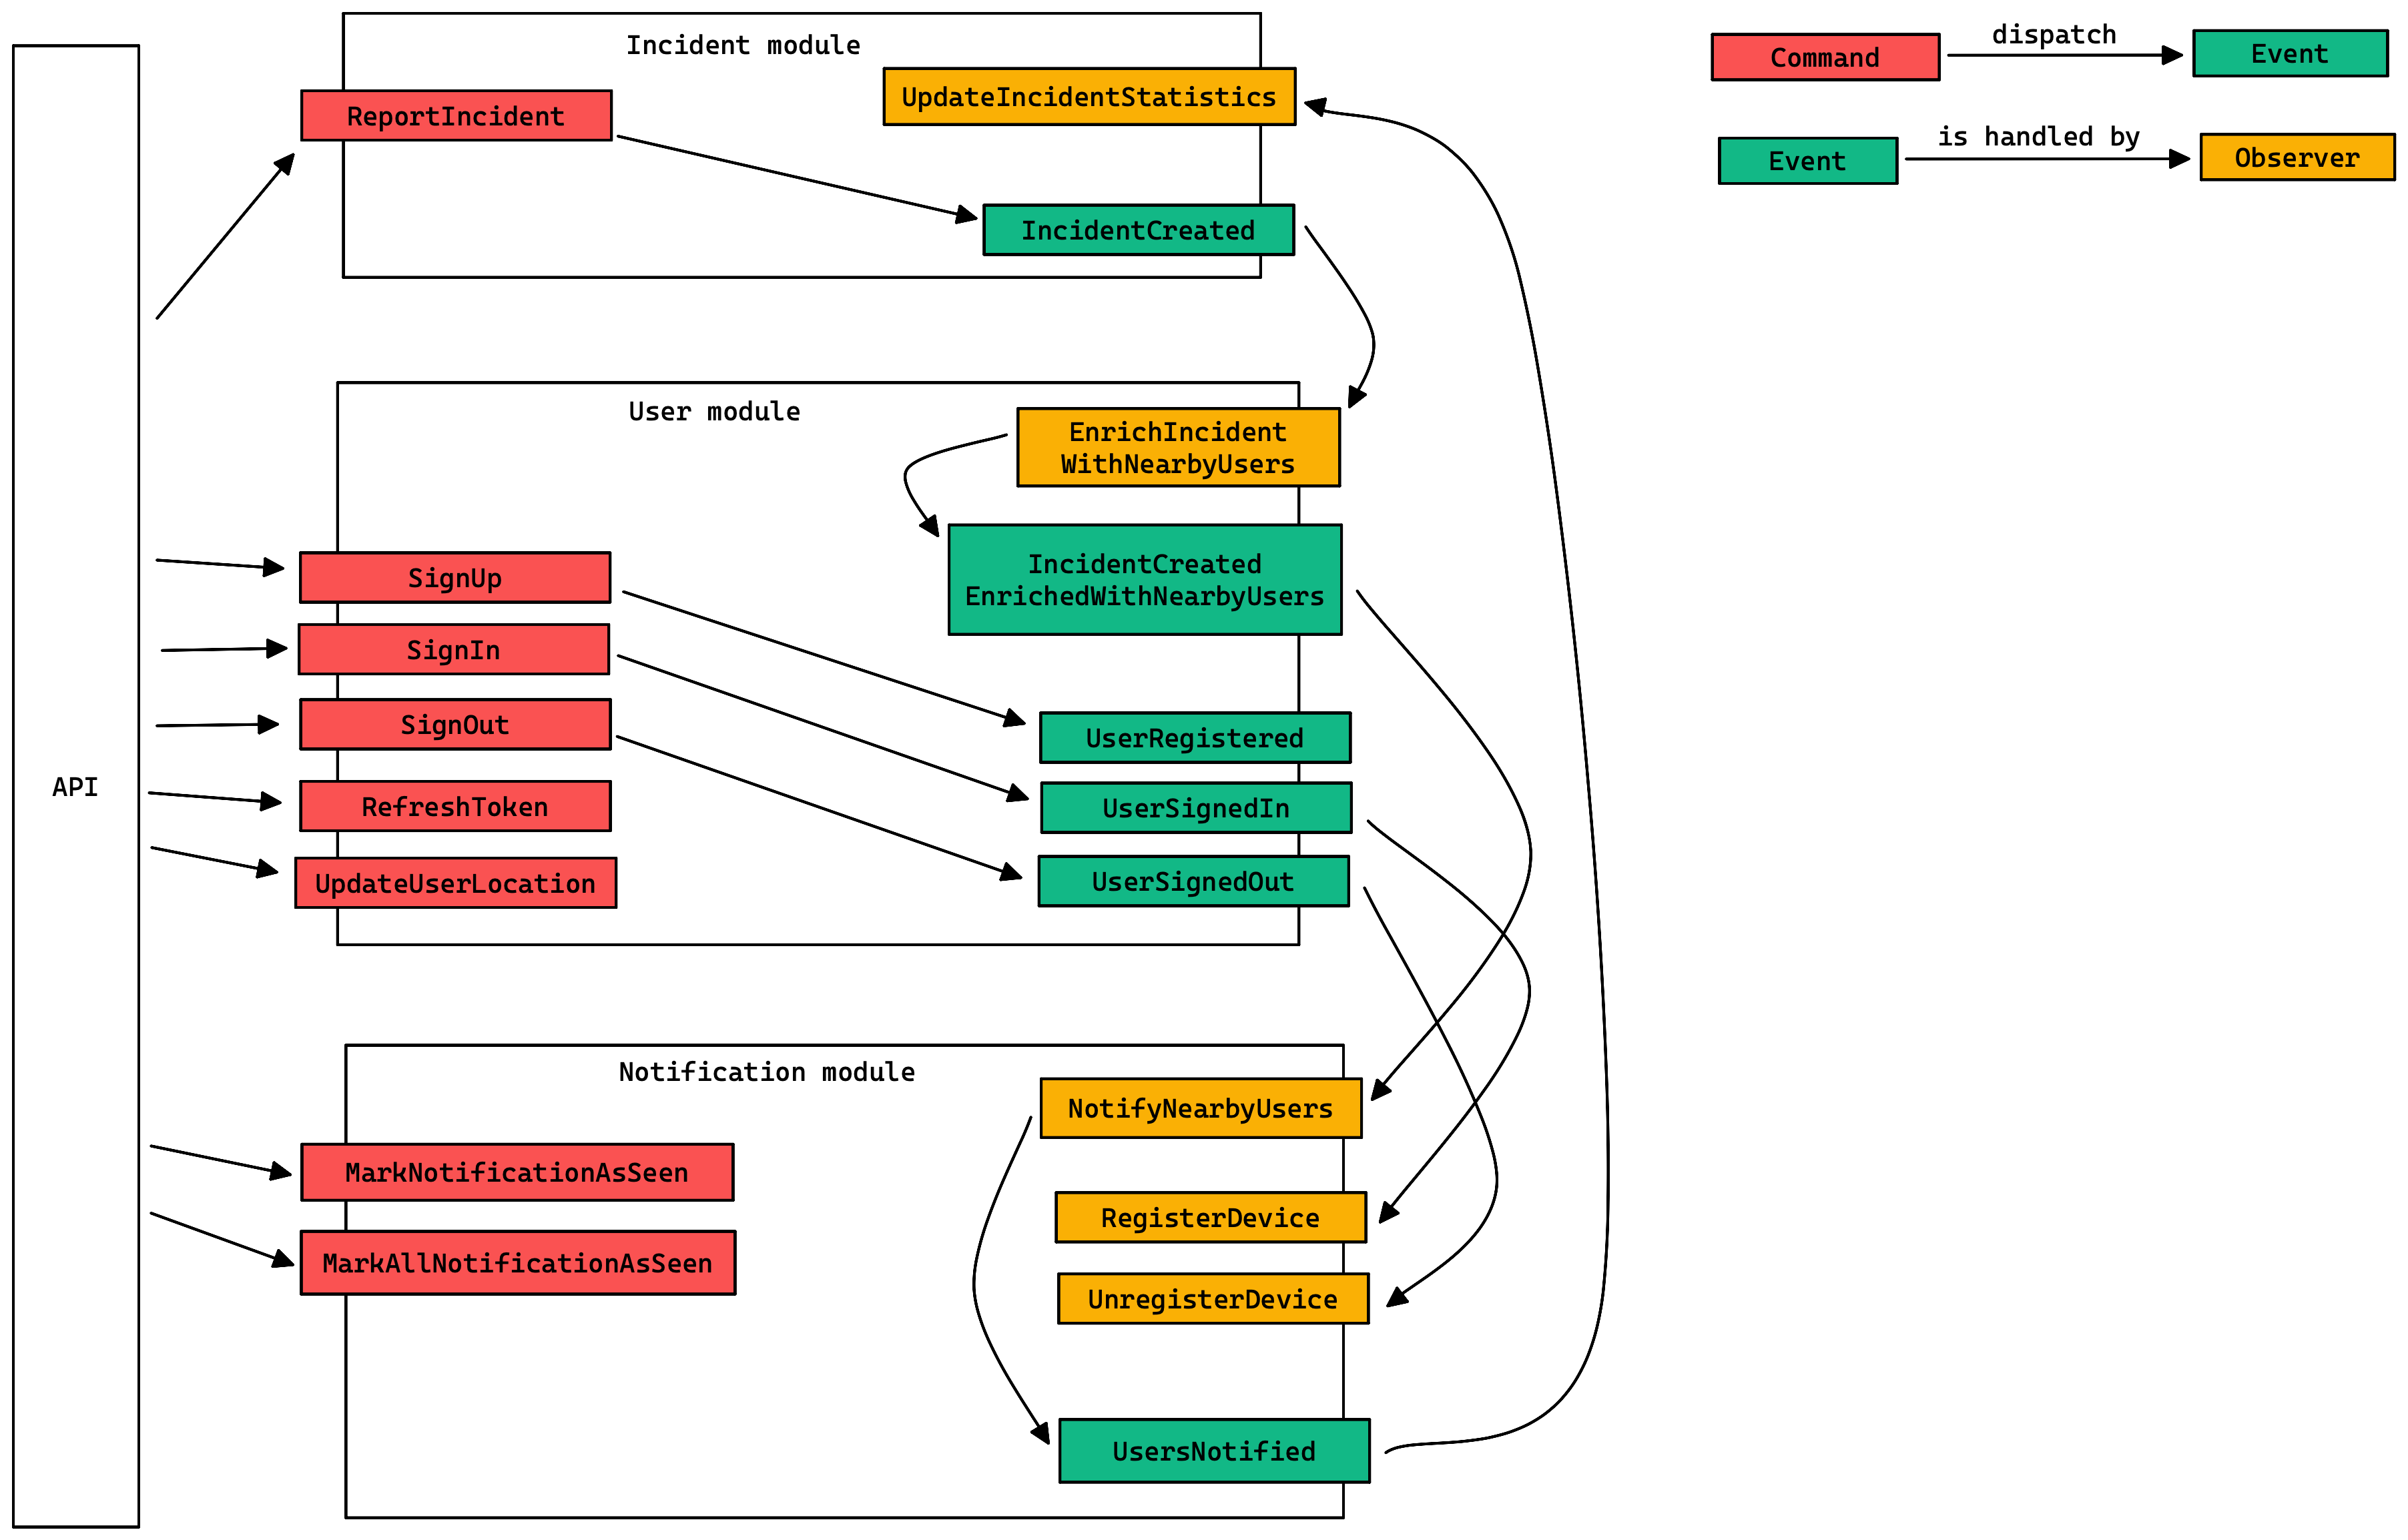
\includegraphics[width=\textwidth]{../diagrams/out/system_server_all_modules_commands-observers-events.png}
	\label{f.system_server_all_modules_commands-observers-events}
	\legend{\small Fonte: Elaborado pelo autor.}
\end{figure}

% \subsubsection{Módulo de incidentes}
% \label{s.servidor-modulo-incidentes}

% \subsubsection{Módulo de usuários}
% \label{s.servidor-modulo-usuarios}

% \subsubsection{Módulo de notificações}
% \label{s.servidor-modulo-notificacoes}

% \section{Aplicativo}
% \label{s.aplicativo}

% telas

% permissoes com SO

% O aplicativo requer qpermissões de acesso ao
